\documentclass{article}
\usepackage[utf8]{inputenc} % Codificación de caracteres
\usepackage{graphicx}
\usepackage{listings}
\graphicspath{ {images/} }

\title{Tipos de Datos mutables e inmutables}
\author{Valery Triana}
\date{\today} % Fecha actual


\begin{document}
\maketitle

\section{Java}

\subsection{Introducción}
A continuación se presentan los tipos de datos primitivos en Java y sus características.
A continuación se presentan los tipos de datos primitivos en Java y sus características.
hola

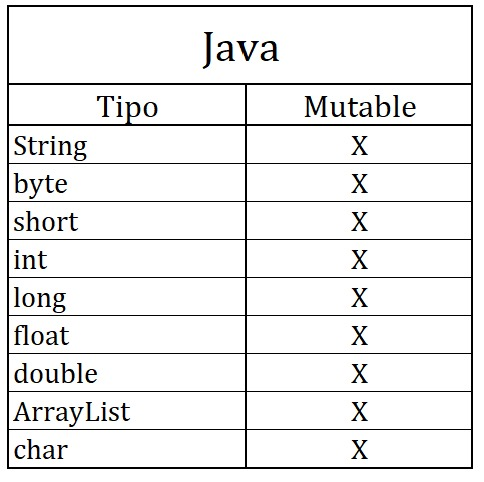
\includegraphics[width=0.5\textwidth]{javaTabla.jpg} % Ajusta el ancho según sea necesario

\subsection{Codigo de ejemplo}

El codigo a continuacion es insertionSort que es un algoritmo de ordenamiento iterativo

\begin{lstlisting}[language=Java, caption=Ejemplo de código en Java]

public static void insertionSort(int[] arr) {
    int n = arr.length;
    for (int i = 1; i < n; ++i) {
        int key = arr[i];
        int j = i - 1;
        while (j >= 0 && arr[j] > key) {
            arr[j + 1] = arr[j];
            j = j - 1;
        }
        arr[j + 1] = key;
    }
}
\end{lstlisting}
\subsection{Uso de tipos de datos mutables o inmutables}
En este ejemplo se puede observar cómo los índices de la variable "arr" se modifican para ordenar el arreglo, lo que refleja un comportamiento mutable.


\subsection{complejidad Temporal del Algoritmo}
En este ejemplo, la complejidad temporal es \( O(n^2)\), Donde n representa la cantidad de elementos en la lista. Esta complejidad surge de la forma en que el algoritmo ordena los elementos, donde en el peor de los casos cada elemento se compara con todos los demás en la lista.

\subsection{Profiling}
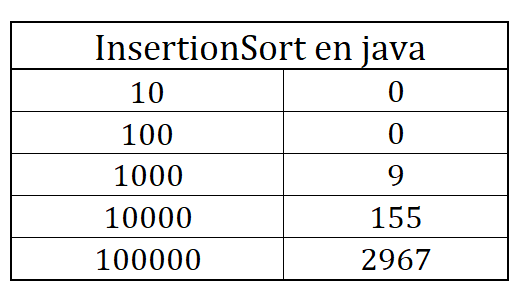
\includegraphics[width=0.5\textwidth]{vsjavaTabla.png}
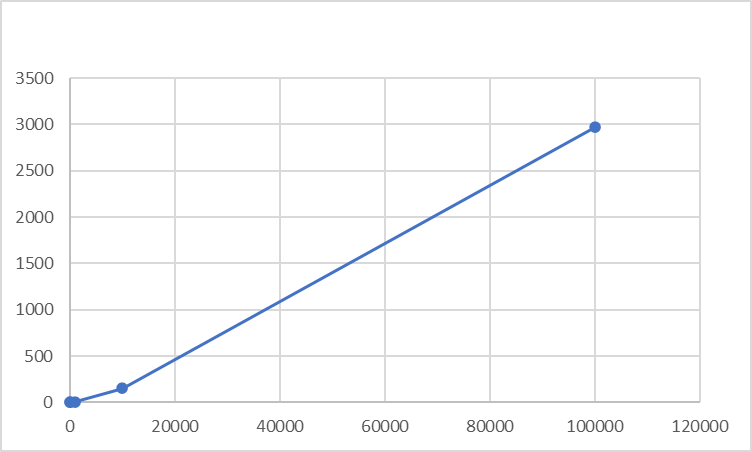
\includegraphics[width=0.5\textwidth]{javaGrafica.png}

\section{Golang}
\subsection{Introducción}
A continuación se presentan los tipos de datos primitivos en Golang y sus características.

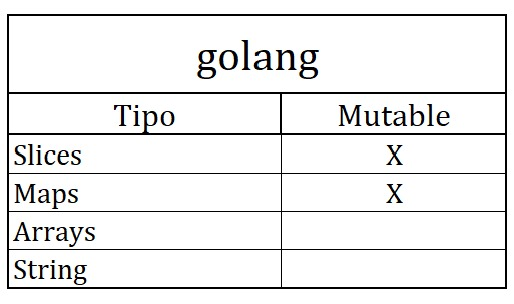
\includegraphics[width=0.5\textwidth]{golangTabla.jpg}

\subsection{Codigo de ejemplo}

El codigo a continuacion se encarga de revisar si existen elementos repetidos en una lista.

\begin{lstlisting}[language=Golang, caption=Ejemplo de código en Golang]
func hasDuplicates(arr []int) bool {
    seen := make(map[int]bool)
    for _, num := range arr {
        if seen[num] {
            return true
        }
        seen[num] = true
    }
    return false
}

\end{lstlisting}
\subsection{Uso de tipos de datos mutables o inmutables}
Podemos ver como el map es un elemento mutable ya que por cada elemento vamos añadiendolo al map y asi mismo editando su valor indicando que ya existe.


\subsection{complejidad Temporal del Algoritmo}
En este ejemplo, la complejidad temporal es O(n), donde n representa la cantidad de elementos en la lista. Esto se debe a que al agregar cada elemento a un mapa, podemos encontrar una coincidencia sin necesidad de comparar todos los elementos entre sí.

\subsection{Profiling}

\begin{lstlisting}[language=Java, caption=Ejemplo de código en Java]

public static boolean hasDuplicates(int[] arr) {
    Map<Integer, Boolean> seen = new HashMap<>();
    for (int num : arr) {
        if (seen.containsKey(num)) {
            return true;
        }
        seen.put(num, true);
    }
    return false;
}
\end{lstlisting}

\subsection{Comparación tiempos de ejecucion}
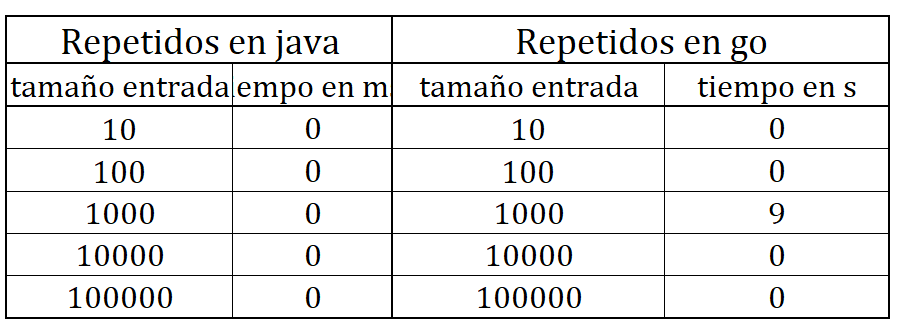
\includegraphics[width=0.5\textwidth]{golangvsjavaTabla.png}
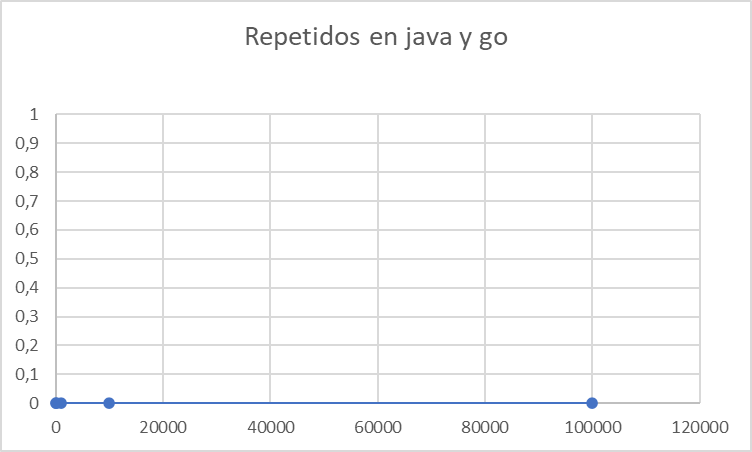
\includegraphics[width=0.5\textwidth]{golangvsjavaGrafica.png}



\section{Python}
\subsection{Introducción}
A continuacion se presenta el algoritmo de búsqueda binaria en Python que es  eficiente para encontrar un elemento en una lista ordenada. Divide repetidamente la lista en mitades y descarta la mitad incorrecta en función de la comparación del elemento medio con el elemento buscado. Esto reduce el espacio de búsqueda a la mitad en cada paso, lo que lo hace rápido incluso en listas grandes.

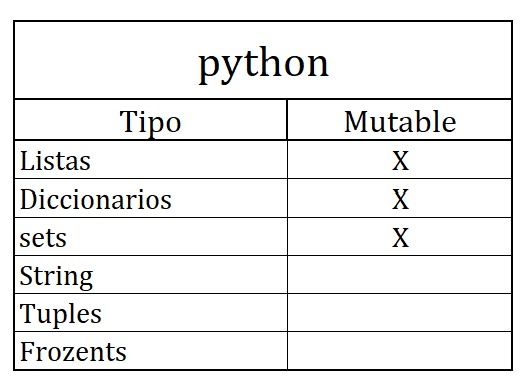
\includegraphics[width=0.5\textwidth]{pythonTabla.jpg}
\subsection{Codigo de ejemplo}
\begin{lstlisting}[language=Python, caption=Ejemplo de código en Python]
def binary_search(arr, x):

    left, right = 0, len(arr) - 1

    while left <= right:
        mid = (left + right) // 2

        if arr[mid] == x:
            return mid

        elif arr[mid] < x:
            left = mid + 1

        else:
            right = mid - 1

    return -1

\end{lstlisting}

\subsection{Uso de tipos de datos mutables o inmutables}
En este caso, las variables left y right son de tipo entero (int), lo que las hace variables mutables. Se utilizan para avanzar en la lista, actualizando continuamente las partes recorridas de la misma al modificar sus valores.

\subsection{Complejidad Temporal del Algoritmo}
La búsqueda binaria tiene una complejidad de O(log(n)), ya que en cada iteración descarta la mitad de todos los elementos de la lista de entrada. Esto se debe a que la lista está ordenada, lo que permite este comportamiento eficiente en términos de tiempo.

\subsection{Profiling}

\begin{lstlisting}[language=Java, caption=Ejemplo de código en Java]

public static int binarySearch(int[] arr, int x) {
    int left = 0;
    int right = arr.length - 1;

    while (left <= right) {
        int mid = (left + right) / 2;

        if (arr[mid] == x) {
            return mid;
        } else if (arr[mid] < x) {
            left = mid + 1;
        } else {
            right = mid - 1;
        }
    }

    return -1;
}
\end{lstlisting}

\subsection{Comparación tiempos de ejecucion}
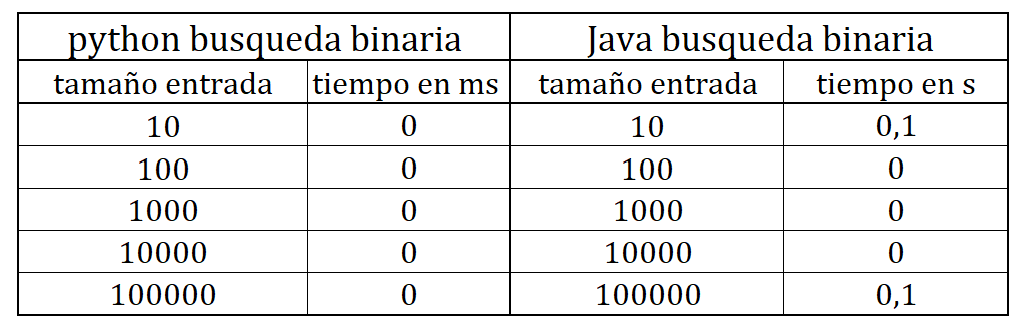
\includegraphics[width=0.5\textwidth]{pythonvsjavaTabla.png}
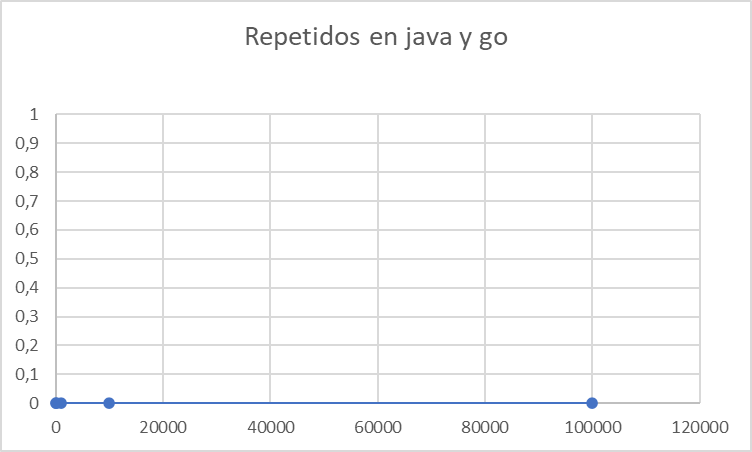
\includegraphics[width=0.5\textwidth]{golangvsjavaGrafica.png}

\section{C++}
\subsection{Introducción}
A continuación se presentan un algoritmo iterativo que dado un numero returna su factorial

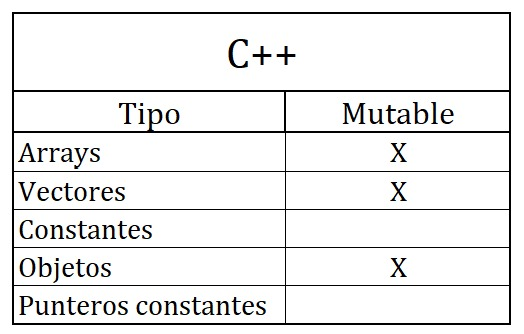
\includegraphics[width=0.5\textwidth]{c++Tabla.jpg}

\subsection{Codigo de ejemplo}
\begin{lstlisting}[language=C++, caption=Ejemplo de código en C++]

unsigned long long factorial(unsigned int n) {
    unsigned long long result = 1;
    for (unsigned int i = 1; i <= n; ++i) {
        result *= i;
    }
    return result;
}

\end{lstlisting}

\subsection{Uso de tipos de datos mutables o inmutables}
En este ejemplo, se define al principio del procedimiento la variable "result", que es mutable. En cada iteración del bucle, esta variable se modifica para calcular y almacenar el factorial del número dado.


\subsection{Complejidad Temporal del Algoritmo}
En este ejemplo, la complejidad temporal es O(n), donde n representa el número de entrada. El algoritmo recorre de 1 hasta n multiplicando su valor para calcular el factorial del número dado. La complejidad lineal se debe a que cada iteración del bucle aumenta linealmente con respecto al tamaño de la entrada.


\subsection{Profiling}

\begin{lstlisting}[language=Java, caption=Ejemplo de código en Java]
    public static long factorial(int n) {
        long result = 1;
        for (int i = 1; i <= n; ++i) {
            result *= i;
            }
    return result;
    }
\end{lstlisting}

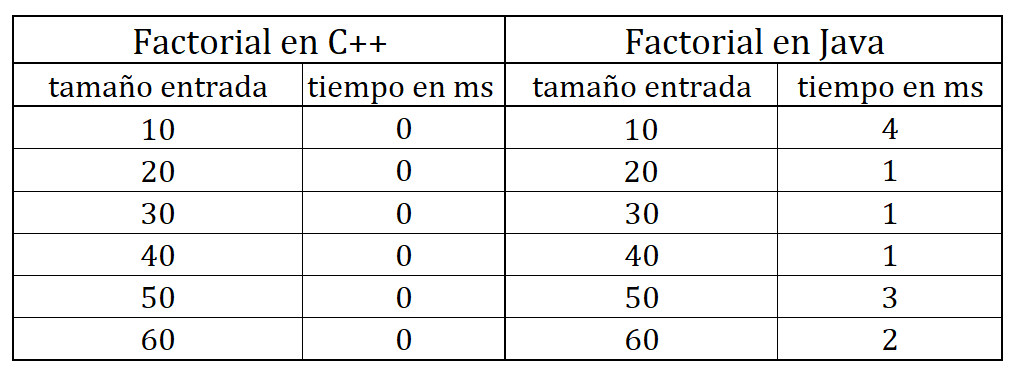
\includegraphics[width=0.5\textwidth]{c++vsjavaTabla.png}
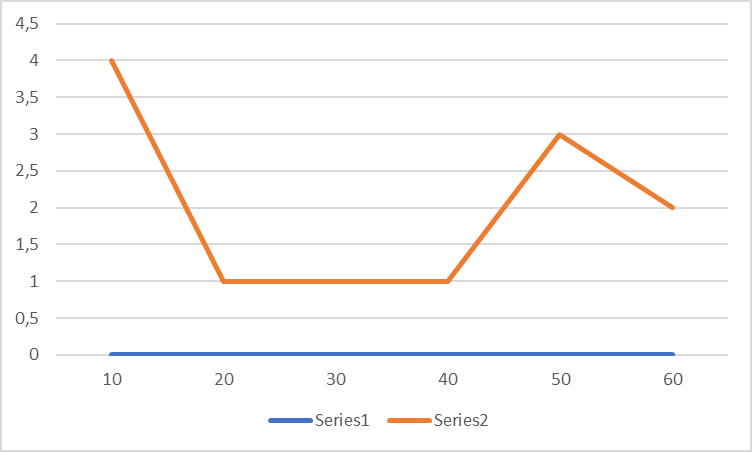
\includegraphics[width=0.5\textwidth]{c++vsjavaGrafica.png}

\end{document}